\documentclass[spanish,xcolor=dvipsnames,svgnames]{beamer}

\mode<presentation>
{
  \usetheme{Warsaw}
  \useoutertheme[subsection=false]{miniframes}
  \setbeamercovered{transparent}
  \usecolortheme[RGB={74,6,94}]{structure}
}

\usepackage{listings}
\usepackage[spanish]{babel}
\usepackage[utf8]{inputenc}
\usepackage[T1]{fontenc}
%\usepackage{lmodern}
%\usepackage{microtype}
\usepackage{xspace}
%\usepackage{ctable}
%\usepackage{tikz}
%\usepackage{alltt,multicol}
%\usepackage{eurosym}
%\usepackage{url}
%\usepackage{etex}
%\usetikzlibrary{chains,positioning,shadows}

\lstset{
  language=C++,
%  frame=Ltb,
%  framerule=0pt,
  aboveskip=0.1cm,
  gobble=6,
%  frame=shadowbox,
%  framextopmargin=0.5pt,
%  framexbottommargin=0.5pt,
%  framexleftmargin=-1cm,
%  framesep=2pt,
%  rulesep=.0pt,
%  backgroundcolor=\color{gray},
%  rulesepcolor=\color{black},
  %
%  stringstyle=\ttfamily,
%  showstringspaces = false,
  basicstyle=\scriptsize\ttfamily,
  morecomment=[l]{//},
%  alsoletter={\&},
%  morekeywords={\&}
%  commentstyle=\color{blue},
%  keywordstyle=\bfseries,
  %
%  numbers=left,
%  numbersep=15pt,
%  numberstyle=\tiny,
%  numberfirstline = false,
%  breaklines=true,
}

% minimizar fragmentado de listados
%\lstnewenvironment{listing}[1][]
%   {\lstset{#1}\pagebreak[0]}{\pagebreak[0]}
% \lstdefinestyle{consola}
%   {basicstyle=\scriptsize\bf\ttfamily,
%    backgroundcolor=\color{gray75},
%   }

\setbeamertemplate{navigation symbols}{}
\addtobeamertemplate{block begin}{\setlength{\textwidth}{1.02\textwidth}}{}
\setbeamersize{text margin left = 2em}

%\newcolumntype{M}[1]{>{\centering}m{#1}}
%\newcommand{\reduce}{\fontsize{8}{9}\selectfont}

%\newcommand{\anotacion}[1]%
%{\(\leftarrow\) \textnormal{\emph{#1}}}

\newcommand{\freemc}{\textit{FreeMicroChat }}

\title[PECS]%
{\freemc \\ Chat sencillo en  C++}


\author[Bueno,Labrador,Tejero]{Aarón Bueno Villares,\\Inmaculada Labrador del Río  y\\ Juan Antonio Tejero Fernández}

\institute[UCA]{
  \begin{small}Universidad de Cádiz\end{small} \\ \bigskip \bigskip
  \begin{normalsize}Programación en entornos cliente-servidor\end{normalsize} \\ \smallskip
}

%\date[19 de enero de 2012]{19 de enero de 2012}

\AtBeginSection[]
               {
                 \begin{frame}<beamer>
                   \frametitle{Índice}
                   \tableofcontents[currentsection]
                 \end{frame}
               }

\begin{document}

\begin{frame}
  \titlepage
\end{frame}

\begin{frame}{Índice}
  \tableofcontents
\end{frame}

\section{Introducción}

\begin{frame}{Introducción}
  \begin{block}{Por qué un chat}
    \begin{itemize}
        \item Pyton, alto nivel.
        \item Otro lenguaje de programación.
    \end{itemize}
  \end{block}
\end{frame}

\begin{frame}{Introducción}
  \begin{block}{Pilares de la aplicación}
    \begin{itemize}
    \item Asincronía
    \item Delegación de funciones
      \begin{itemize}
      \item Callback functions
      \end{itemize}
    \end{itemize}
  \end{block}
  \begin{figure}[h]
    \centering
    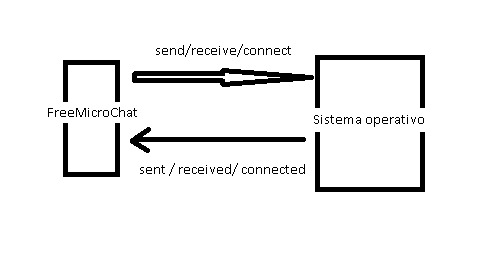
\includegraphics[width=200pt]{img/Callbacks-funct.png}
    \caption{Delegación y callback}
  \end{figure}
\end{frame}

\begin{frame}{Introducción}
  \begin{block}{Asincronía y chats}
    \begin{itemize}
    \item Toda conversación de chat es asíncrona, pues no se sabe cuándo llegarán mensajes por parte de otro usuario.
    \end{itemize}
  \end{block}
  \begin{block}{Asincronía en FreeMicroChat}
    \begin{itemize}
    \item Boost, Asio
    \end{itemize}
  \end{block}
\end{frame}

\begin{frame}{Introducción}
  \begin{block}{Boost}
    \begin{itemize}
    \item Qué es
      \begin{itemize}
      \item Boost Software License
      \item 40 librerías
      \end{itemize}
    \end{itemize}
  \end{block}
  \begin{block}{Por qué Boost}
    \begin{itemize}
    \item Comunidad viva
    \item Documentación
    \item Empresas y software:
      \begin{itemize}
      \item Adobe Software Libraries
      \item LyX Document Editor
      \item The C++/Tk Library
      \end{itemize}
    \item Librería estándar de C++
    \end{itemize}
  \end{block}
\end{frame}


%%%%%%%%%%%%%%%%%%%%%%%%%%%%%%%%%%%%%%%%%%%%%%%%
\section{Boost::Asio y Serialización}
\begin{frame}{Boost::Asio}
  \begin{block}{Boost::Asio}
    \begin{itemize}
    \item Librería C++ multi-plataforma para redes y programación de E/S
    \end{itemize}
  \end{block}

  \begin{block}{Asincronía con Boost::Asio}
    \begin{itemize}
    \item boost::asio::io\_service
      \begin{itemize}
      \item boost::asio::io\_service::run()
      \end{itemize}

    \end{itemize}
  \end{block}
\end{frame}

\begin{frame}{Secuencia de eventos en operaciones asíncronas}
  \begin{figure}[h]
    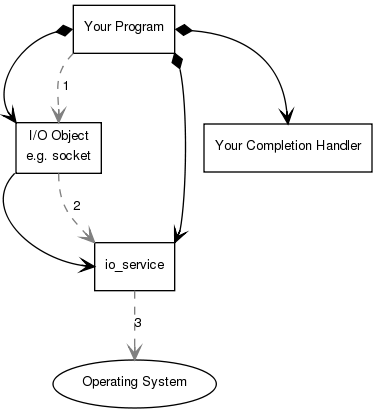
\includegraphics[width=165pt]{img/async_op1.png}
    \caption{Fase 1}
  \end{figure}
\end{frame}

\begin{frame}{Secuencia de eventos en operaciones asíncronas}
  \begin{figure}[h]
    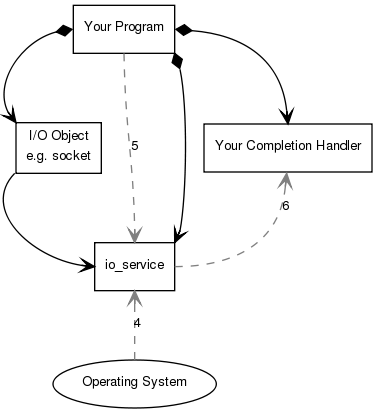
\includegraphics[width=165pt]{img/async_op2.png}
    \caption{Fase 2}
  \end{figure}
\end{frame}

\begin{frame}{Arquitectura de \freemc}
\begin{block}{}
  \begin{figure}[h]
    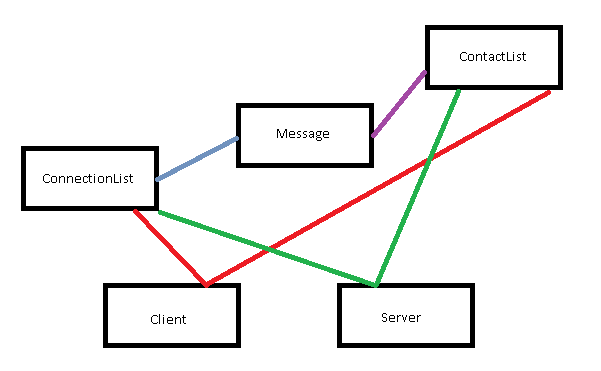
\includegraphics[width=250pt]{img/Arquitectura.png}
    \caption{Clases y sus relaciones}
  \end{figure}
\end{block}
\end{frame}

\begin{frame}[fragile]{Algunos detalles técnicos extra}
  \begin{block}{Serialización (boost::serialization)}
    \begin{itemize}
    \item Codificación a formato tratable.
    \item Usado ampliamente para transporte red.
    \item Otros usos: hacer persistente un/os dato/s en ejecución.
    \end{itemize}
  \end{block}

  \begin{block}{Serialización en \freemc}
    \begin{lstlisting}[language=C++]
      string Message::serialize() const
      {
        ostringstream oss;
        text_oarchive ar(oss);

        ar << *this;

        return oss.str();
      }
    \end{lstlisting}
  \end{block}
\end{frame}

\begin{frame}{Algunos detalles técnicos extra}
  \begin{block}{Hilos (boost::thread)}
      \begin{itemize}
      \item Crea un hilo para ejecutar una función.
      \item boost::thread myThread(nombre\_function);
      \item boost::thread\_group
      \end{itemize}
  \end{block}

  \begin{block}{Binding (boost::bind)}
    \begin{itemize}
    \item Transporta una función en forma de objeto a función.
    \item Número indeterminado de parámetros y parámetros anónimos.
    \item Ejemplo: boost::bind(\&Server::\_newClient, this, id, \_1)
    \end{itemize}
  \end{block}

\end{frame}

\begin{frame}{Algunos detalles técnicos extra}

  \begin{block}{Punteros compartidos (boost::shared\_ptr)}
    \begin{itemize}
    \item Contador del número de veces que se ha copiado el puntero.
    \item Se borra automáticamente (\textit{delete}) cuando se haya
      borrado la última copia.
    \end{itemize}
  \end{block}

  \begin{block}{Algunas cosas de C++11}
    \begin{itemize}
    \item \textit{auto}: auto i = fibonnacci(5);
    \item \textit{decltype}: decltype(fibonnacci(5)) i =
      fibonnacci(5);
    \item Bucles basados en rango: for (auto \&i: myVector) cout << i <<
      endl;
    \end{itemize}
  \end{block}

\end{frame}


%%%%%%%%%%%%%%%%%%%%%%%%%%%%%%%%%%%%%%%%%%%%%%

\section{Implementación}

\begin{frame}{Implementación}
  \begin{block}{Puntos que trataremos}
    \begin{itemize}
    \item Conexión entre servidor y cliente
    \item Envío de nick; formalizar conexión
    \item Conversacion
    \end{itemize}
  \end{block}
  \pause

  \begin{block}{Como servidor central}
    \begin{itemize}
    \item Desde un punto de vista lógico, servirá como concentrador de conexiones.
    \end{itemize}
  \end{block}
  \begin{block}{Como puente entre cliente}
    \begin{itemize}
    \item Un mensaje de un cliente a otro, pasando por el servidor.
    \end{itemize}
  \end{block}
\end{frame}

%% \begin{frame}{Servidor con doble funcionalidad}

%% \end{frame}

\begin{frame}[fragile]{Servidor central: Conexión entre cliente y servidor}

  \begin{block}{void Server::up(), void Server::\_connectionControl()}
    \begin{lstlisting}[language=C++]
      // Server configure: reuse_address, listen, pasive.

      unsigned id = _contactList.addPhantomContact();
      _connectionList.newConnection(id);

      async_accept(*_connectionList.getSocket(id),
                   bind(&Server::_newClient, this, id, _1));

      _service->run();
    \end{lstlisting}
  \end{block}

  \begin{block}{void Client::start()}
    \begin{lstlisting}[language=C++]
      // Configure query: protocol, ip, port.
      _connectionList.connect(_idConnection, query); // Synchronous.

      _talkLoop();
      _service->run();
    \end{lstlisting}
  \end{block}

\end{frame}

\begin{frame}[fragile]{Servidor central: recepción/envío de nicks}
  \begin{block}{void Server::\_newClient(unsigned id)}
    \begin{lstlisting}[language=C++]
      // Called function after establishing connection.
      _connectionList.recvMsg(id, &Server::_getNick, this);
      _connectionControl();
    \end{lstlisting}
  \end{block}

  \pause

  \begin{block}{void Client:::\_talkLoop()}
    \begin{lstlisting}[language=C++]
      Message nick(Message::MSG_NICK, _nick);

      _connectionList.sendMsg(_idConnection, &Client::_sentNick,
                              this, nick);
      _connectionList.recvMsg(_idConnection,
                              &Client::_recvContactList, this);
    \end{lstlisting}
  \end{block}
\end{frame}

\begin{frame}[fragile]{Servidor centra: recepción/envío de nicks}
  \begin{block}{void Server::\_getNick(unsigned id, Message msg)}
    \begin{lstlisting}[language=C++]
      _contactList.checkinPhantomContact(id, msg.message());
      _broadcastContactList();
      _connectionList.recvMsg(id, &Server::_newMsg, this);
    \end{lstlisting}
  \end{block}

  \pause

  \begin{block}{void Client::\_recvContactList(unsigned id, Message msg)}
    \begin{lstlisting}[language=C++]
      _contactList.deserialize(msg.message());
      _connectionList.recvMsg(id_my_socket, &Client::_newMsg, this);
      _threads.create_thread(bind(&Client::_readMsg, this));
    \end{lstlisting}
  \end{block}

  \pause

  \begin{block}{void Client::\_newMsg(unsigned id, Message msg)}
    \begin{lstlisting}[language=C++]
      _contactList.deserialize(msg.message());

      _connectionList.recvMsg(id_my_socket, &Client::_newMsg, this);
    \end{lstlisting}
  \end{block}

\end{frame}

\begin{frame}[fragile]{Servidor como puente:  Conversación}
   \begin{block}{Client 1: void Client::\_readMsg()}
     \begin{lstlisting}[language=C++]
       // Print prompt, message queue and reading from keyboard.
       Message msg(MSG_NORMAL, str, id_nick_target);
       _connectionList.sendMsg(my_id, &Client::_sentMsg, this, msg);
     \end{lstlisting}
   \end{block}

   \pause

   \begin{block}{void Server::\_newMsg(unsigned id, Message msg)}
     \begin{lstlisting}[language=C++]
       Message newMsg(MSG_NORMAL, msg.message(), id);
       _connectionList.sendMsg(msg.target(), &Server::_sentMsg, this,
                               newMsg);
       _connectionList.recvMsg(my_id, &Client::_newMsg, this);
     \end{lstlisting}
   \end{block}

   \pause

   \begin{block}{Client 2: void Client::\_newMsg(unsigned id, Message msg)}
     \begin{lstlisting}[language=C++]
       // Read new message in a local stream os.
       _messageQueue.push(os.str());
       _connectionList.recvMsg(my_id, &Client::_newMsg, this);
     \end{lstlisting}
   \end{block}
\end{frame}


\begin{frame}[fragile]{Servidor como puente: conversación}

  \begin{block}{template<class F, class O> \\ void
      ConnectionList::recvMsg(unsigned id, F f, O o)}
    \begin{lstlisting}[language=C++]
      async_read_until(*getSocket(id), *getRecvBuffer(id), '\0',
                       bind(&ConnectionList::_recvMsg<F, O>,
                            this, id, f, o, _1, _2));
    \end{lstlisting}
  \end{block}

  \begin{block}{template<class F, class O> \\
    void ConnectionList::sendMsg(unsigned id, F f, O o, Message msg)}
    \begin{lstlisting}[language=C++]
      async_write(*getSocket(id), *buffer,
                  bind(&ConnectionList::_sendMsg<F, O>,
                       this, id, f, o, msg, _1, _2))
    \end{lstlisting}
  \end{block}
\end{frame}

%%%%%%%%%%%%%%%%%%%%%%%%%%%%%%%%%%%%%%%%%%%
\section{Ejecución}
\begin{frame}{}
  \begin{block}{A chatear}
    \begin{itemize}
    \item Veámos a \freemc en acción...
    \end{itemize}
  \end{block}

\end{frame}


%%%%%%%%%%%%%%%%%%%%%%%%%%%%%%%%%%%%%%%%%%%

\section{Conclusiones}
\begin{frame}{}
  \begin{block}{¿Qué hemos aprendido?}
    \begin{itemize}
    \item Hemos aprendido la comunicación entre sockets a un nivel un poco más bajo que al visto en clase.
    \item Hemos aprendido a usar una librería potentísima: Boost::Asio.
    \item Hemos aprendido a implmentar un chat sencillo C++.
    \end{itemize}
  \end{block}
\end{frame}

%%%%%%%%%%%%%%%%%%%%%%%%%%%%%%%%%%%%%%%%%%%
\begin{frame}{Fin de la presentación}
  \begin{center}
    {\huge Muchas gracias por su atención}

    \vspace{.1\textheight}

  \end{center}
\end{frame}

\end{document}
